\section{Analyse Technique}

\subsection{Présentation}

\subsubsection{Histoire de l'analyse technique}
Les sources de l'analyse technique remonte au XVIIIème siècle quand les Japonais essayaient d'anticiper l'évolution des cours du riz. Ensuite, on retrouve trace de l'analyse technique au début du XXème siècle grâce aux recherches de Richard Dow. Au début, l'analyse technique était purement graphique mais désormais on retrouve une grande part d'outil mathématiques. \\

A partir des années 30, Ralph Nelson Elliot a mis en évidence les fameuses vagues d'Elliot. Nous retrouvons également d'autres grands noms associés à l'analyse technique tels que Steve Nison, réputé pour la méthode des chandeliers, Stan Weinstein, pour les moyennes mobiles et John Bollinger. \\


\subsubsection{Définition}
Tentant de définir l’analyse technique, John Murphy disait : « L’analyse technique est l’étude de l’évolution d’un marché, principalement sur la base de graphiques, dans le but de prévoir les futures tendances ». L'analyse technique correspond à l'étude des graphiques des cours de la bourse ainsi que de divers indicateurs déduits de ces cours. Grâce à cette étude, le but est d'essayer d'anticiper l'évolution future des cours. \\

L'analyse technique peut s'appliquer à tout types de marchés : indices, actions, taux, matières premières. Les mêmes méthodes pouvant être appliqués dans tous les cas. 

L'analyse technique repose sur trois hypothèses fondamentales :
\begin{itemize}
\item Le prix intègre toute l'information disponible
\item Les prix évoluent en tendance
\item L'histoire se répète
\end{itemize}


\subsubsection{Différents courants}

Au fur et à mesure de l'histoire, l'analyse technique a évolué et s'est perfectionné. C'est ainsi que l'on peut distinguer quatre principaux courants dans l'analyse technique moderne :
\begin{itemize}
\item \textbf{Analyse technique chartiste} repose sur l'étude des cours et historique avec la recherche de motifs se répétant.  
\item \textbf{Analyse technique statistique} repose essentiellement sur l'étude de la modélisation de l'évolution des cours.
\item \textbf{Les vagues d'Elliot} cherchent à décomposer le cours comme étant une fractale.
\item \textbf{Le market profile} consiste en une étude statistique des cours, repose sur l'hypothèse d'une loi normale pour les cours. 
\end{itemize}

\subsection{Différents outils}
Dans la partie précédente nous avons vu qu'au cours de l'histoire l'analyse technique n'avait cessé d'évoluer au fur et à mesure des découvertes. Nous allons présenté dans cette partie quatre outils d'analyse technique que nous allons mettre à disposition de l'utilisateur dans notre jeu. \\

\subsubsection{Les chandeliers}
Les chandeliers ou chandelier Japonais est un type de graphique utilisé en analyse technique pour représenter les variations d'un cours. \\

Les informations nécessaires à leur tracé sont au nombre de quatre: les cours d'ouverture, de clôture, le plus haut et le plus bas de la séance. Cette technique fait apparaître une notion supplémentaire; si le cours a baissé pendant la période, le chandelier est noir, si le cours a monté, le chandelier est blanc. le corps rectangulaire représente l'intervalle entre le cours d'ouverture et le cours de fermeture. Les deux traits fins noirs à chaque bout du corps sont les évolutions extrêmes de la journée. On les appelle les ombres hautes et basses. 

\begin{figure}[H]
  \center
  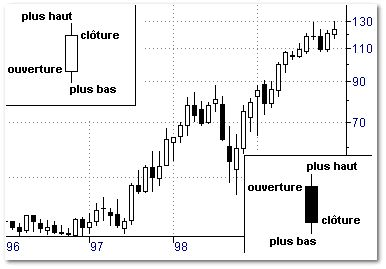
\includegraphics[scale=0.5]{../graph/chandelier.png}
  \caption{Exemple de graphique avec des chandeliers}
\end{figure}

 La désignation pour le chandelier blanc (marché haussier) est le Yang (yo-sen ), pour le chandelier noir (marché baissier) le Yin (in-sen). \\
 
Normalement, après une bougie avec un corps long on ne doit pas prendre position sauf si on est dans un contexte haussier pour une bougie blanche ou contexte baissier pour une bougie noire. 

Pour effectuer des prévisions à partir des chandeliers, il faut être capable de repérer des figures significatives : 
\begin{itemize}
\item  \textbf{Ligne perçante} : représente un retournement. Un long corps de baisse suivi d’un long corps de hausse. Le trait horizontal représente le milieu de la bougie de baisse, la bougie de hausse doit clôturer au-dessus de ce trait.  
\begin{figure}[H]
  \center
  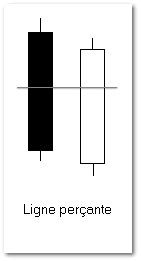
\includegraphics[scale=0.5]{../graph/chandelier1.png}
  \caption{Exemple de ligne perçante}
\end{figure} 

\item \textbf{Ciel ouvert} : condition inverse de la ligne perçante. Un long corps de hausse suivi d’un long corps de baisse. Le corps de baisse ouvre au-dessus du milieu de la bougie de hausse. Ce motif représente un retournement également. 
\begin{figure}[H]
  \center
  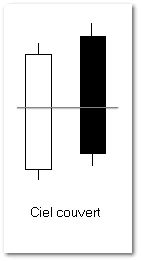
\includegraphics[scale=0.5]{../graph/chandelier2.png}
  \caption{Exemple de ciel ouvert}
\end{figure} 

\item \textbf{Le marteau} : il présage d’une hausse si il arrive au cours d’une baisse. Il n’y a pas d’ombre au dessus et une très longue en dessous, il peut s’agir d’une bougie noire ou blanche la signification est la même .
\begin{figure}[H]
  \center
  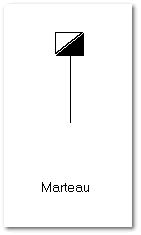
\includegraphics[scale=0.5]{../graph/chandelier3.png}
  \caption{Exemple de marteau}
\end{figure} 

\item \textbf{Le pendu} : il présage d’une baisse si il arrive au cours d’une hausse. Les couleurs n’ont pas d’importance. 
 \begin{figure}[H]
  \center
  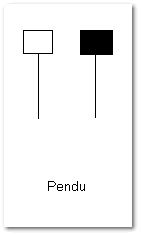
\includegraphics[scale=0.5]{../graph/chandelier4.png}
  \caption{Exemple de pendu}
\end{figure} 

\item \textbf{Les englobantes} : Elles peuvent être haussières ou baissières et sont très puissantes. Si la baissière arrive après une hausse significative ou la haussière après une baisse significative, on assistera probablement à un retournement.
\begin{figure}[H]
  \center
  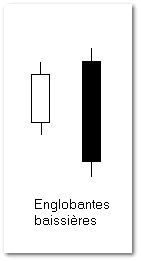
\includegraphics[scale=0.5]{../graph/chandelier5.png}
  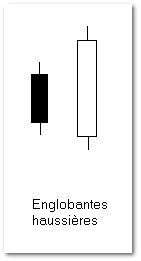
\includegraphics[scale=0.5]{../graph/chandelier6.png}
  \caption{Exemple d'englobante}
\end{figure} 

\item \textbf{Étoile du soir et étoile du matin} : l’étoile du soir indique un retournement possible à la baisse et l’étoile du matin indique au contraire un retournement possible à la hausse.
\begin{figure}[H]
  \center
  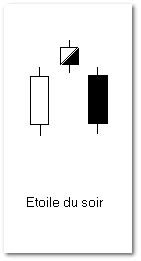
\includegraphics[scale=0.5]{../graph/chandelier7.png}
  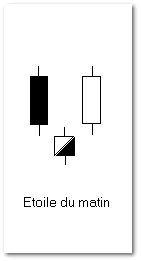
\includegraphics[scale=0.5]{../graph/chandelier8.png}
  \caption{Exemple d'étoile du soir et d'étoile du matin}
\end{figure} 

\item \textbf{Les dojis} : Ils sont très simples à reconnaître : un seul trait horizontal indiquant que les cours de clôtures et d’ouvertures sont les mêmes. Il existe plusieurs types de doji. Le \textbf{doji simple} un long trait vertical de chaque côté de la barre horizontal indique de l’indécision. Les \textbf{dojis dragons}, sont composés d’un long trait sous la barre horizontale, les cours ont beaucoup baissés dans la journée pour se maintenir finalement. Le \textbf{doji pierre tombale} est l’inverse du doji dragon. Si plusieurs dojis se suivent : séance suivante très évolutive.
\begin{figure}[H]
  \center
  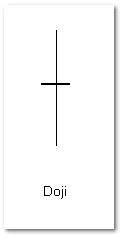
\includegraphics[scale=0.5]{../graph/chandelier9.png}
  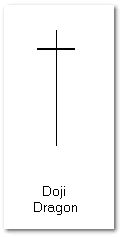
\includegraphics[scale=0.5]{../graph/chandelier10.png}
  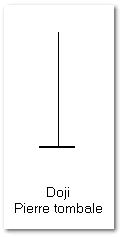
\includegraphics[scale=0.5]{../graph/chandelier11.png}  
  \caption{Exemple de dojis}
\end{figure} 
\end{itemize}

\subsubsection{Les moyennes mobiles}

\subsubsection{Les Bollinger}

\subsubsection{Les volumes}


